    \subsection{Server Side}\label{Server Side Design}
    In this section we are going to introduce the design, implementation and configuration that we have done on the server side. In section~\ref{Server Introduction} we introduce the framework that we have built upon and what we are going to do with it. Next follows use cases, in section~\ref{Server Use Cases}. Section~\ref{Description of ESB concepts} will go into more detail about what the framework consists of. The section will also guide you through the basic processing units which is used in the framework. The next section,~\ref{Textual Server Dataflow}, contains the dataflow through the server side, which will help you get a good overview of our design. Section~\ref{Extensions to the ESB} goes into detail in describing our custom components in the framework, and together with the dataflow should give you a good understanding of the whole server side. Together with section~\ref{Server Sequence Diagrams} you should get a good overview of the system. Section~\ref{Configuration of the ESB} will 
give you the details 
about how we 
have configured the framework, it will not contain description of how we have set variables during testing, but using this description should make it possible to get the framework up and running.

    \subsubsection{Introduction}\label{Server Introduction}
    The server side architecture consists of several components, the WSO2 ESB, the Monitoring Service and the GlassFish server. The GlassFish server is not necessary to modify and the MS is something we must assume to exist in the network. The ESB is what we have to modify, configure and extend to meet our requirements.

    The ESB will be used to implement QoS for the Web services. To do this, it will have to communicate with the MS, in addition to the clients and the services. The ESB must be configured to work as a proxy for the services on the GlassFish server. It will also be configured to use certain mediation sequences for incoming requests and outgoing responses. The extension to the ESB consists mainly of custom mediators used in the mediation sequences. These mediators have the tasks of determining priority of messages, contacting the MS for bandwidth data, and enforcing the priority. Also modifications to the source code of one of the ESBs libraries were made to allow DiffServ to be set in the IP header.
    
    \subsubsection{Use Cases}\label{Server Use Cases}
    This section outlines the use cases that we have thought of in relation to the server side. With the help of these you should get a rough idea of what we want the server side to be able to do.\\\\
    \textbf{Title:} Request mediation\\
    \textbf{Requirements:} 3, 7\\
    \textbf{Actors:} Client, ESB, GlassFish\\
    \textbf{Main}
    \begin{enumerate}
        \item Client sends SOAP message with SAML Token to ESB proxy
        \item ESB extracts SAML token to get the client role
        \item ESB removes SAML metadata from message
        \item ESB adds metadata to message context.
        \item ESB sends message to GlassFish endpoint
    \end{enumerate}
    \textbf{Extensions:}
    \begin{itemize}
        \item[] 2a. SAML Token is invalid
        \item[] 2b. ESB sends error message to client
    \end{itemize}
    \textbf{Precondition:}
    \begin{itemize}
        \item Client is connected to ESB
    \end{itemize}
    \\
    \textbf{Title:} Response mediation \\
    \textbf{Requirements:} 2, 3, 7\\
    \textbf{Actors:} Client, ESB, GlassFish \\
    \textbf{Main}
    \begin{enumerate}
        \item GlassFish sends message to ESB
        \item ESB sets priority metadata in message context and SOAP header.
        \item ESB retrieves bandwidth information (See Monitoring Service communication use case)
        \item ESB prioritizes message (See Prioritize message use case)
        \item ESB sends message to Client
    \end{enumerate}
    \textbf{Extensions:} \\
    \textbf{Precondition:}
    \begin{itemize}
        \item Request mediation
    \end{itemize}
    \\
    \textbf{Title:} Monitoring Service communication\\
    \textbf{Actors:} Monitoring Service(MS), ESB\\
    \textbf{Main}
    \begin{enumerate}
        \item ESB requests bandwidth information from MS to a specific address
        \item MS returns bottleneck bandwidth to the ESB, as well as an identifier for the last \gls{tr} before the endpoint.
    \end{enumerate}
    \textbf{Extensions:}
    \begin{itemize}
        \item[]	1a. ESB specifies an invalid address
        \item[]	2a. MS returns no information
        \item[]	2b. Address is in the same sub net as the ESB
    \end{itemize}
    \textbf{Precondition:}
    \begin{itemize}
        \item Response mediation
    \end{itemize}
    \\
    \textbf{Title:} Prioritize messages\\
    \textbf{Requirements:} 2, 6, 8\\
    \textbf{Actors:} ESB\\
    \textbf{Main}
    \begin{enumerate}
        \item ESB acquires QoS information through settings
        \item ESB adds QoS information to the SOAP header of the message
        \item ESB sets DiffServ field in IP header
    \end{enumerate}
    \textbf{Extensions:}\\
    \textbf{Precondition:}
    \begin{itemize}
        \item Response mediation
        \item Monitoring Service communication
    \end{itemize}

    \subsubsection{Description of ESB concepts}\label{Description of ESB concepts} 

    In this section we briefly describe some important concepts of the ESB and message mediation.

    A mediator is the basic processing unit in \gls{synapse}\footnote{\gls{synapse} - An enterprise service bus. [\url{http://synapse.apache.org/}]}. Each message going through the ESB gets mediated through a sequence of mediators, which can be configured through either XML or WSO2’s graphical user interface. As long as the mediator inherits from a Synapse interface, any custom mediator can be used in the same manner as the built in mediators. To control the flow of messages through the ESB, there are two paths that can be controlled, the “in sequence” and the “out sequence”, which can also be configured to only apply for certain endpoints.

    The ESB is built around the notion of a message context, this object contains all the information regarding the message and the context around it. In the message context we can add properties, manipulate the message itself and manipulate the sending streams of the message. All the properties added during the receiving of a message are also added to the outgoing message, which we can use to our advantage.

    Each mediator in the sequence gets access to the message context of the incoming or the outgoing message and can thus manipulate the context to its liking. When the mediator is done with the work it is supposed to do, it either calls the next mediator, sending it the possibly altered message context or returning true to indicate that the work is done.
    
    We have taken full advantage of the modularity in the ESB. This means that even though much of the functionality in our mediators could be moved into one or two mediators we have decided to make many. For us this means much easier testing of each component and it gives each mediator a more clearly defined role. For our customer this means an easier setup where they can mix and match each mediator and easily create custom sequences with just the functionality they need.

    \subsubsection{Dataflow}\label{Textual Server Dataflow} 
        This section describes the data flow through the ESB with the help of two diagrams. As a bonus, these diagrams show the general architecture of the server side very well.
\\
        \begin{figure}[h]
            \centering
            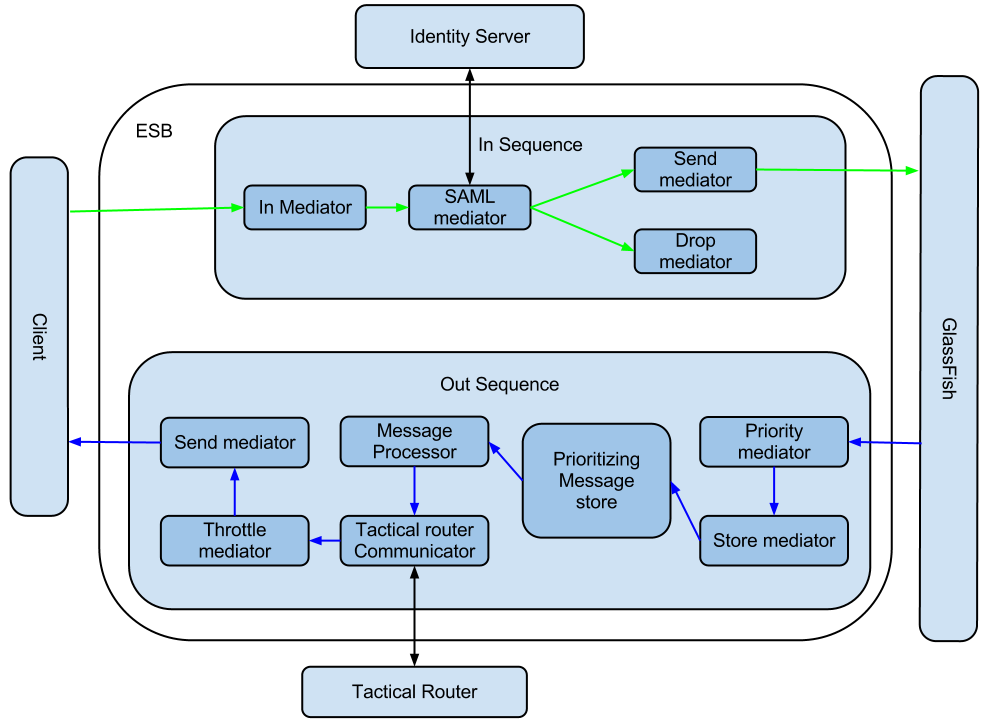
\includegraphics[width=\textwidth]{DataFlowDiagramServer}
            \caption{Server Data Flow}
            This diagram shows how the data flows through the server side. 
            \label{fig:DataFlowDiagramServer}
        \end{figure}
\\
Service Request :\\
To follow this flow, trace the green arrows in Fig:~\ref{fig:DataFlowDiagramServer}. The ESB receives a request message from a Client, it is then sent to the SAML mediator, and then to the InMetadata mediator which when done sends it to the service endpoint on the GlassFish server, and the flow is over.
\\\\
Service Response:\\
To follow this flow, trace the blue arrows in Fig:~\ref{fig:DataFlowDiagramServer}. The ESB receives a response message from the Service, it is then sent through a sequence of mediators, first the OutMetadata mediator, SoapPriority mediator, MS mediator and then  the Store mediator. The Store mediator stores the message in the Prioritized Message Store. The message is stored until the Sampling Message Processor picks it out before sending it on to another sequence of mediators. First in the sequence is the DiffServ mediator, then the Throttle Mediator and finally the Send mediator. The send mediator sends the message back to the client and the flow is completed.
\\
    \begin{figure}[h]
        \centering
        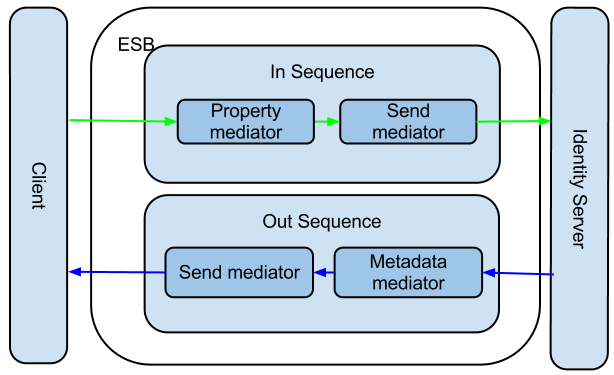
\includegraphics[width=\textwidth]{SAMLauthenticationflow}
        \caption{SAML Authentication Flow}
        This describes the flow of an authentication request. 
        \label{fig:SAMLauthenticationflow}
    \end{figure}
\\           
SAML Authentication Request:\\
This flow is shown in Fig:~\ref{fig:SAMLauthenticationflow}.The ESB receives a request (from a Client) directed at the dummy Identity Server, the ESB then uses the SendBack mediator to send the same message it got in back. The message then travels to the Out sequence where it gets a priority, a DiffServ value and some metadata gets added to the header of the message. The reason why this is done is explained in section~\ref{Changes:IS}.

    \subsubsection{Extensions to the ESB}\label{Extensions to the ESB} 
    This section contains a textual description of all the mediators used in the ESB. First we describe all the custom mediators and then follows a short description of the built-in mediators we use. All of our custom mediators have an accompanying sequence diagram to give a detailed overview of their inner working which is referenced in the title.
\\\\
\textbf{Custom mediators:}\\\\
SAML mediator(Fig:~\ref{fig:SAMLmediator}):\\
    This mediator retrieves the user role from the SAML authentication and sets this as a property in the message context. The service is retrieved from the 'recipient' field also found in the SAML authentication and added as another property. Depending on the configuration of the ESB this mediator can also detach the SAML authentication if this is no longer needed.
\\\\
InMetadata mediator(Fig:~\ref{fig:InMetadatamediator}):\\
	This mediator adds the IP of the client to the message context, which is done in order for the MS mediator to do its work. It will also set the Time-to-Live values in the message context if this is present in the SOAP header.
\\\\
OutMetadata mediator(Fig:~\ref{fig:OutMetadatamediatorsequencediagram}):\\
    This mediator retrieves the client role and service properties from the message context. These properties are then used along with a persistent registry to infer a priority for the message, and what the DiffServ field in the IP header should be set as. The priority and DiffServ values are then set as new properties in the message context.
    The DiffServ property in the message context will be used in the synapse core to set the DiffServ field before sending the message (See appendix~\ref{Server Setup Guide}).
\\\\
SoapPriority mediator(Fig:~\ref{fig:SoapPrioritymediator}):\\
	This mediator adds the DiffServ value and the priority as two custom SOAP header items. We use these fields on the client side in order for the clients to use the same DiffServ value.
\\\\
MS mediator(Fig:~\ref{fig:MSmediatorsequence}):\\
    This mediator retrieves the \gls{ipaddress}\footnote{\gls{ipaddress} - A numerical label assigned to each device connected to the Internet} of the receiving client from the endpoint reference in the message context. It sends this IP address to the Monitoring Service and gets an identifier for the last \gls{tr} on the path to the client, as well as the limiting bandwidth on the path. The mediator then sets this information as properties in the message context before sending the message to the next mediator.
\\\\
Prioritized Message store:\\
    This is not a mediator, but it is an important part of the response mediation sequence. This is a message store that stores messages in a priority queue. The queue is mainly ordered by the priority property of the message context, and secondly by the time when added. When retrieving messages from this store, the message on the top of the queue is returned. This ensures that high priority messages are processed before lower priority messages.
\\\\
DiffServ mediator(Fig:~\ref{fig:DiffServmediator}):\\
	The DiffServ mediator sets the correct DiffServ value on the socket. The DiffServ value is retrieved from the same value as the OutMetadata mediator put in earlier. Since correct use of DiffServ was very important to the client this mediator also does extensive logging which is important to look at when debugging.
\\\\
Throttle mediator(Fig:~\ref{fig:Throttlemediator}):\\
    This mediator is used to ensure that high priority messages are sent first, by disrupting already sending messages, and it tries to ensure that the network is not being overflowed by this server by holding back messages. To determine what to disrupt and what to hold back, and for how long, several properties are used; the priority of the message, the available bandwidth, the IP address of the client side \gls{tr}, and the real time demand of the request. In order to do this, the mediator must keep a list of sending messages and where those messages are going.
\\\\
SendBack mediator:\\
    This mediator sends the message back to the client, but before it is sent it is mediated through the out sequence of the ESB.
\\\\
\textbf{Built in Mediators:}\\\\
Send mediator:\\
    This is a built in mediator that sends the message to an endpoint (the requested service).
\\\\
Store mediator:\\
    This is a built in mediator that stores the message context in a message store, here this is the Prioritized Message store.
\\\\
Sampling Message Processor:\\
    This is not a mediator. It is a built in class that takes messages out of the Prioritized Message Store at a defined interval. And then sends them to a mediator sequence, here starting with the DiffServ mediator.

    \subsubsection{Sequence Diagrams}\label{Server Sequence Diagrams}
    This section contains some sequence diagrams which can be used to get a more in depth look at the code and methods used in the mediators described in the previous section, \ref{Extensions to the ESB}. None of the diagrams reflects the actual method names or display the full complexity of the code, but it should be easy enough to find and understand the corresponding parts of the source code. The first diagram, Fig:~\ref{fig:System-levelsequencediagram}, shows how communication is between the client, ESB and GlassFish. It is very high level, none of the calls are actually method calls in the system.
    
        \begin{figure}[H]
            \centering
            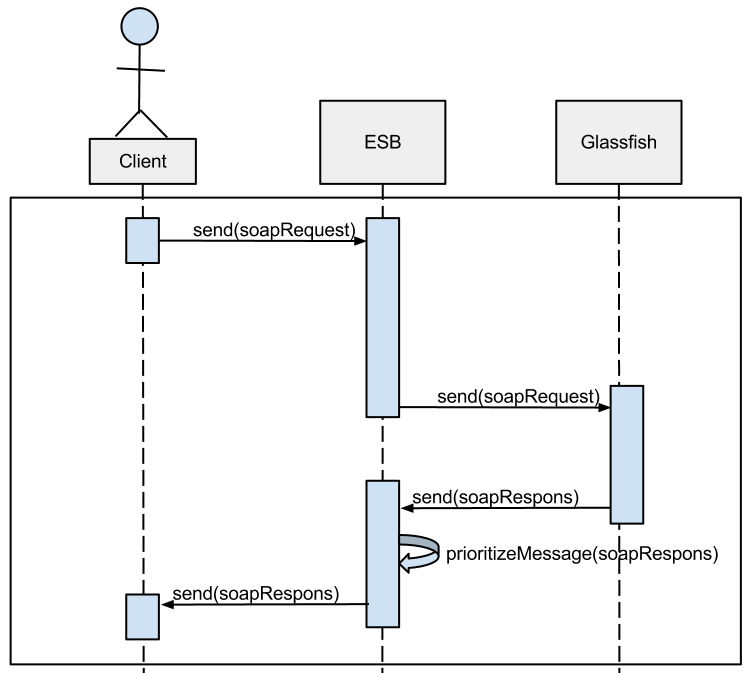
\includegraphics[scale=0.3]{System-levelsequencediagram}
            \caption{System-level sequence diagram}
            This high level diagram shows how the client communicates with Web services through the ESB.
            \label{fig:System-levelsequencediagram}
        \end{figure}
        
        \begin{figure}[H] 
            \centering
            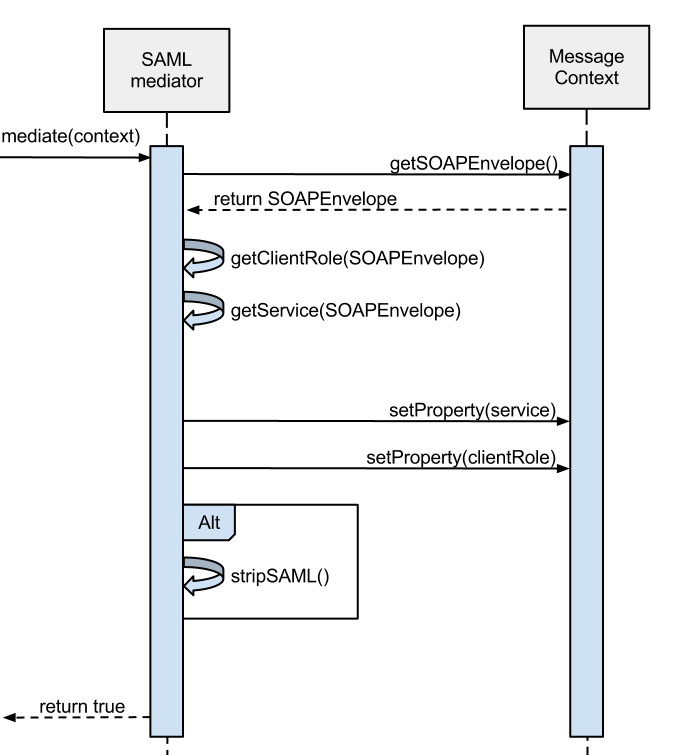
\includegraphics[scale=0.3]{SAMLmediator}
            \caption{SAML mediator sequence diagram}
            This diagram shows how the SAML mediator will get data from the message, and set it in the message context so it can be used later in the response sequence
            \label{fig:SAMLmediator}
        \end{figure}
        
        \begin{figure}[H]
            \centering
            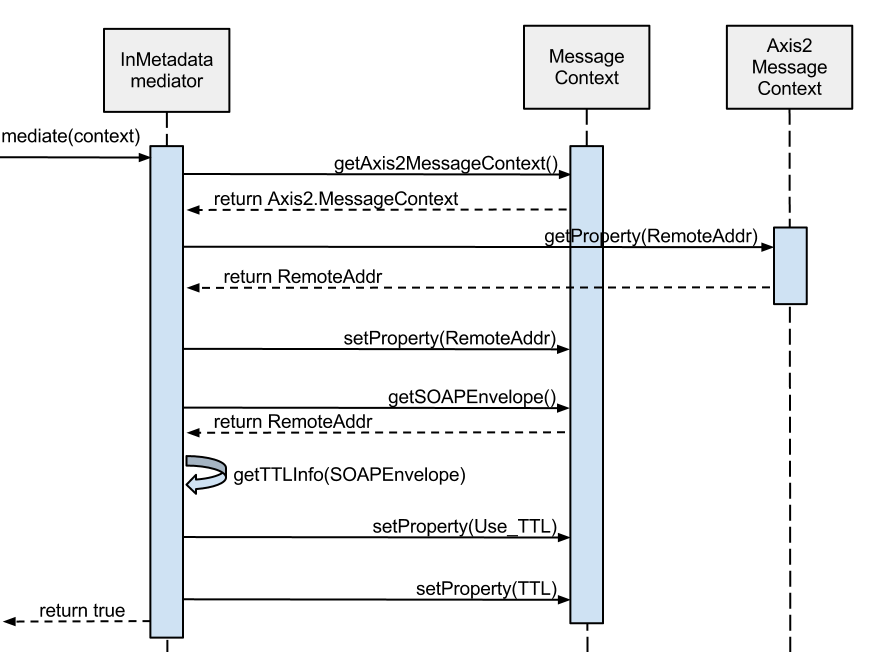
\includegraphics[scale=0.3]{InMetadatamediator}
            \caption{InMetadata mediator sequence diagram}
            This diagram shows how the InMetadata mediator works when it adds the IP address and Time-to-Live.
            \label{fig:InMetadatamediator}
        \end{figure}
        
        \begin{figure}[H]
            \centering
            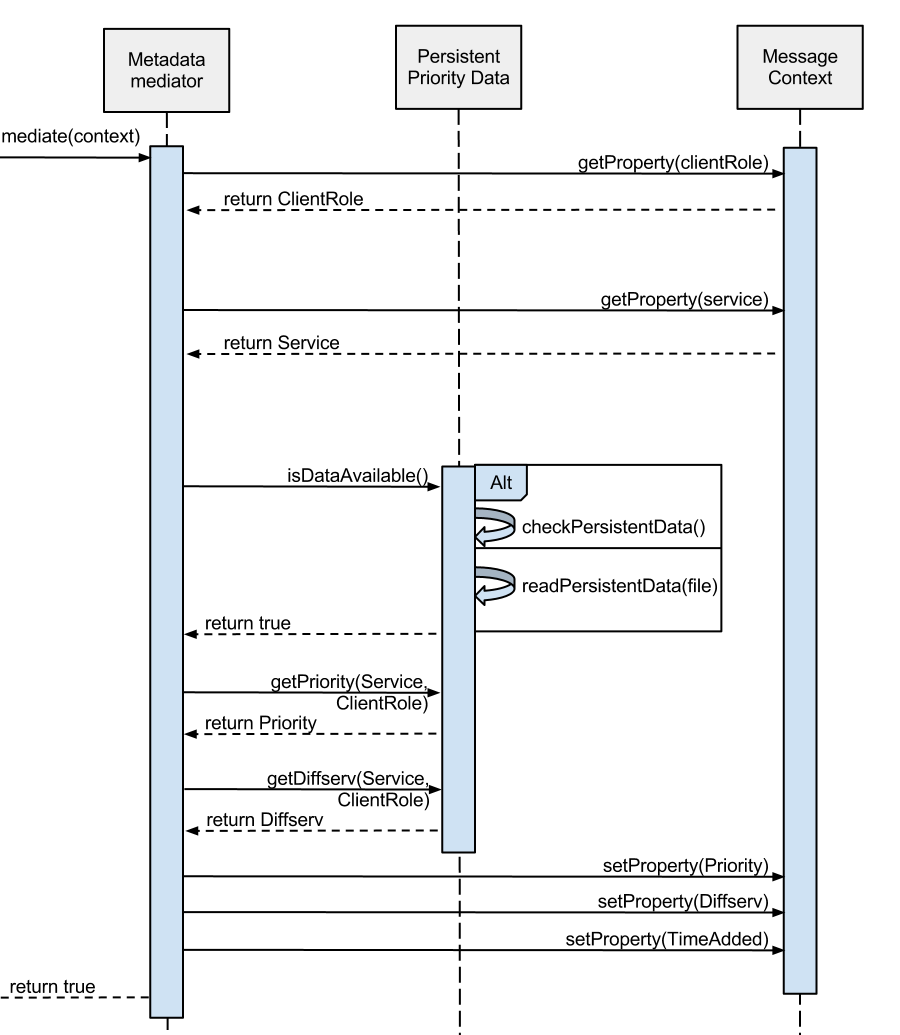
\includegraphics[width=\textwidth]{OutMetadatamediatorsequencediagram}
            \caption{OutMetadata mediator sequence diagram}
            The diagram shows how OutMetadata mediator works.
            \label{fig:OutMetadatamediatorsequencediagram}
        \end{figure}
        
        \begin{figure}[H] 
            \centering
            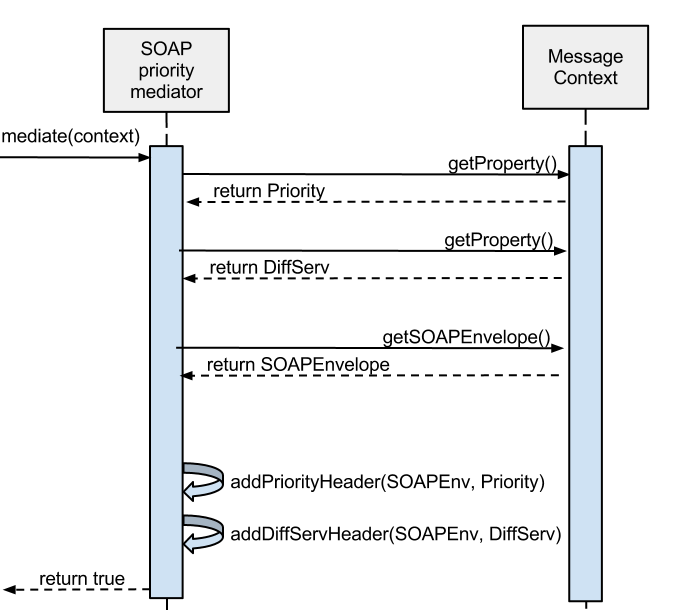
\includegraphics[scale=0.3]{SoapPrioritymediator}
            \caption{SOAP Priority mediator sequence diagram}
            This diagram shows the inner working of the SOAP priority mediator.
            \label{fig:SoapPrioritymediator}
        \end{figure}
    
        \begin{figure}[H] 
            \centering
            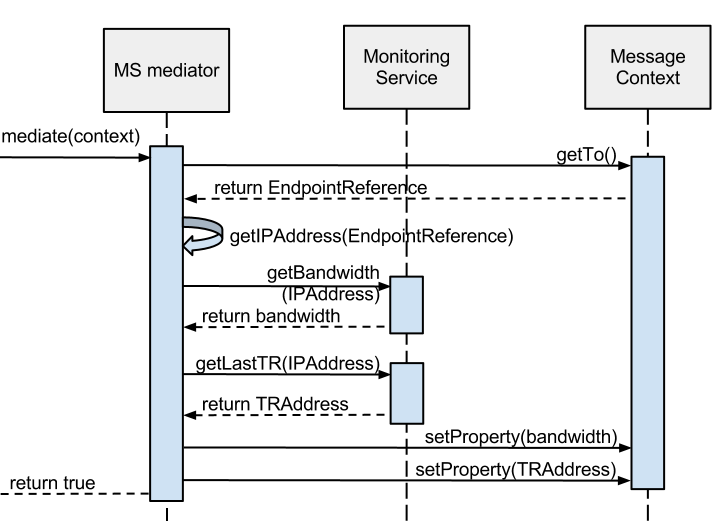
\includegraphics[scale=0.3]{MSmediatorsequence}
            \caption{Metadata mediator sequence}
            This diagram shows how the MS mediator retrieves the routing information from the MSCommunicator and add it to the Message Context.
            \label{fig:MSmediatorsequence}
        \end{figure}
        
        \begin{figure}[H]
            \centering
            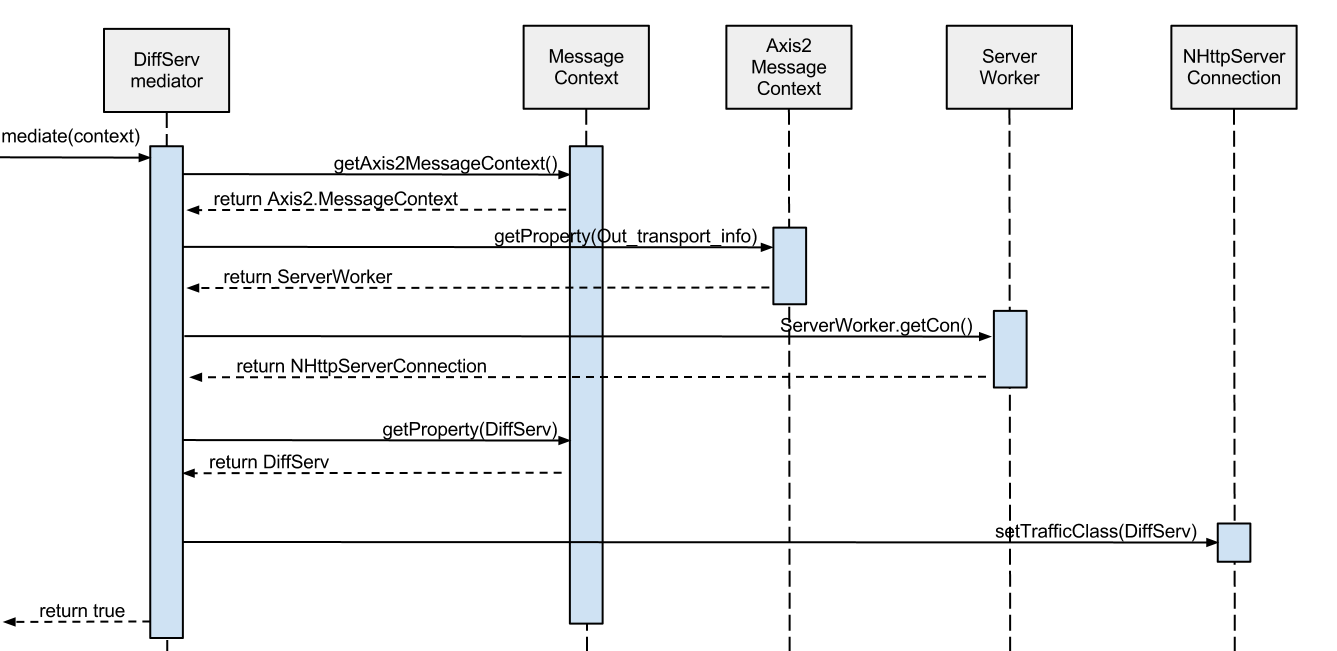
\includegraphics[scale=0.4, angle=270]{DiffServmediator}
            \caption{DiffServ mediator sequence diagram}
            How we set DiffServ priority on the underlying Socket.
            \label{fig:DiffServmediator}
        \end{figure}
        
        \begin{figure}[H] 
            \centering
            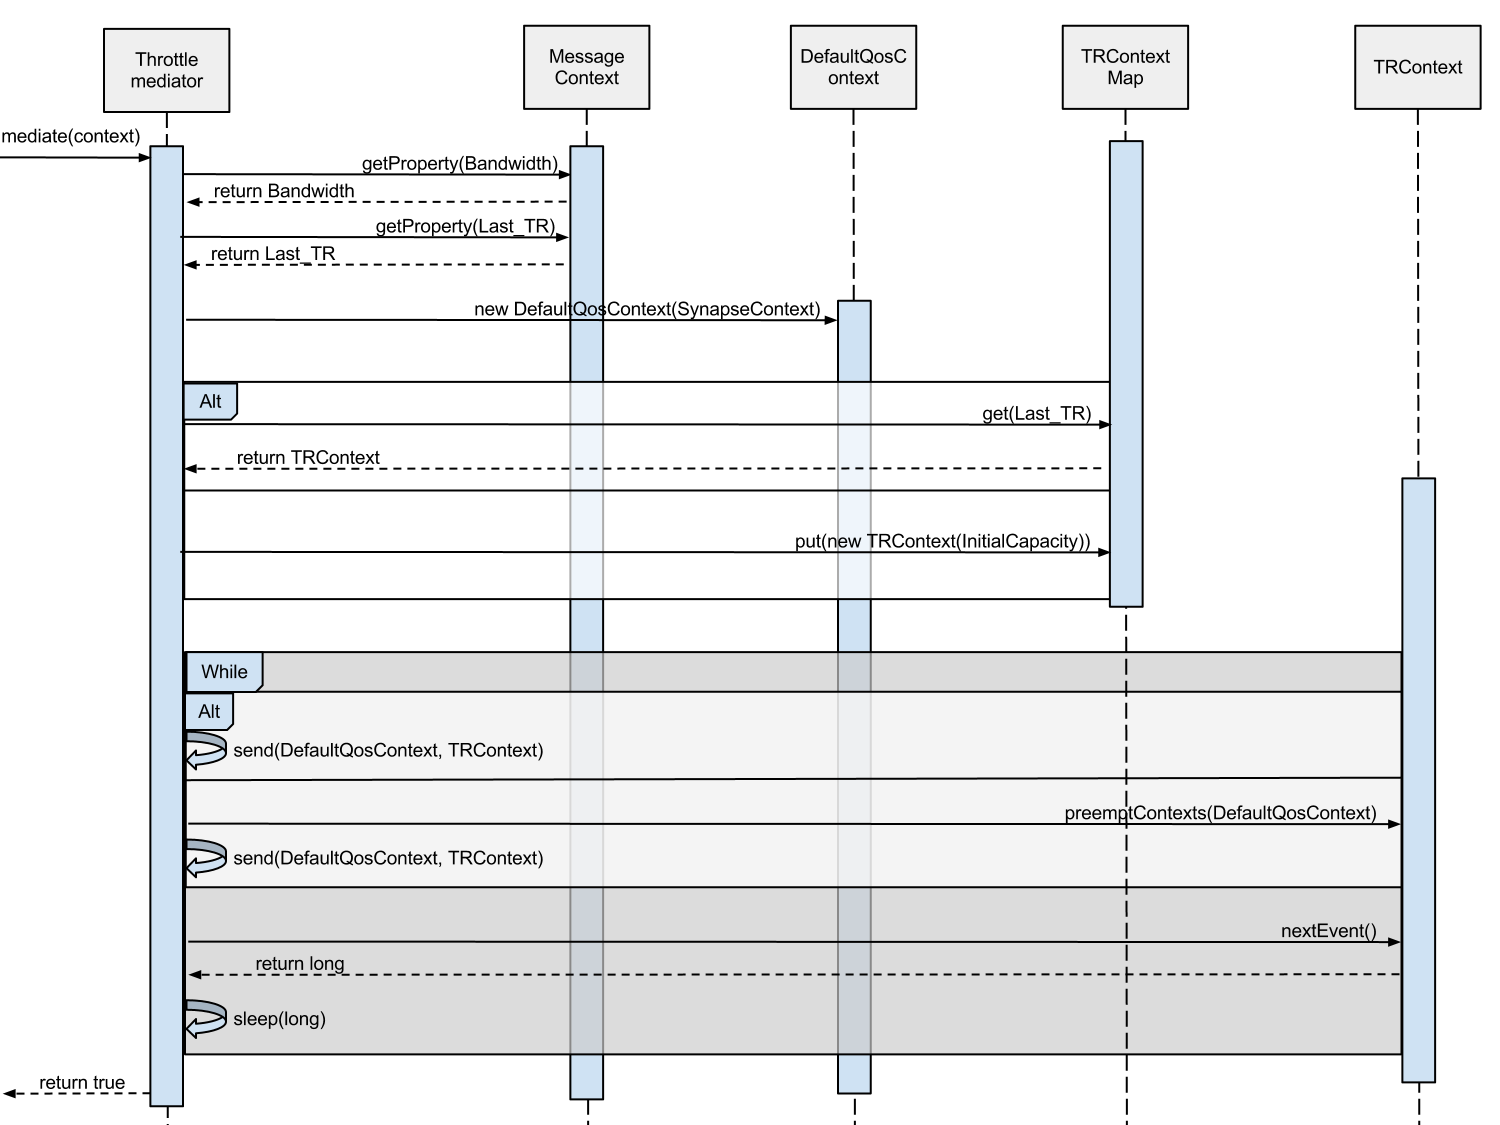
\includegraphics[scale=0.3, angle=270]{Throttlemediator}
            \caption{Throttle mediator sequence diagram}
            The meat of the server side mediators.
            \label{fig:Throttlemediator}
        \end{figure}
        

    \subsubsection{Configuration of the ESB}\label{Configuration of the ESB} 
	In this section we explain how to configure the ESB. For general configuration of the ESB, e.g., configuring new services or WS-Discovery, please refer to the official WSO2 ESB or Apache Synapse documentation.

	\begin{shaded}
	It is highly recommended that you follow appendix~\ref{Server Setup Guide} for an in depth guide on how to setup the ESB with the needed modifications before you read this section.
	\end{shaded}

	First we look at the file “ppd.xml”, which should now be in “/path/to/wso2esb/”, ppd is short for Persistent Priority Data. This file contains maps from “service name” and “client role” to “priority” and “diffserv”. Here “service name” should be the path to the service on the ESB, “client role” should be the name of the client’s role, “priority” is the internal priority we use in the ESB (higher is better) and “diffserv” is the value that will be set in the IP header when communicating with the client. Both DiffServ and priority must be integers.
	The service element also has the useDefault property which, when set to true, lets roles not configured in this file use values in the default role. When useDefault is set to false unconfigured clients will get a priority and DiffServ value of 0. If useDefault is set to false there is no need to configure a default client for the service.
	Below is an example setup of a service in ppd.xml.\\

\lstset{language=XML, style=eclipse}
\lstset{showstringspaces=false}
\begin{lstlisting}[frame=single, caption={ms.xml}, label=ms listing, breaklines=true] %Ok to not have this referenced =)
<?xml version="1.0" encoding="UTF-8" ?>
<config>
   <services>
	   <service name="/services/EchoService" 
	   useDefault="true">
	         <client role="clientRole1">
	           <priority>100</priority>
	           <diffserv>10</diffserv>
	         </client>
	       <client role="Default">
	           <priority>321</priority>
	           <diffserv>8</diffserv>
	       </client>
	   </service>
   </services>
</config>
\end{lstlisting}

	Next we look at a file that is specific to our implementation of the MSCommunicator (Monitoring Service Communicator). Since our implementation does not actually have a monitoring service to contact we use the file “ms.xml” in “/path/to/wso2esb/” to configure data groups of destination IP, name of last \gls{tr} before client and the bandwidth capacity of the ‘weakest’ link on the path measured in KiBps. Below is an example configuration.\\

\lstset{language=XML, style=eclipse}
\lstset{showstringspaces=false}
\begin{lstlisting}[frame=single, caption={ppd.xml}, label=ppd listing, breaklines=true] %It is ok that this is not referenced in text =)
<?xml version="1.0" encoding="UTF-8" ?>
<config>
   <RoutingInfos>
	   <RoutingInfo>
	       <destIP>127.0.0.1</destIP>
	       <lastTR>bob</lastTR>
	       <bandwidth>0.2</bandwidth>
	   </RoutingInfo>
   </RoutingInfos>
</config>
\end{lstlisting}

	If the MSCommunicator is modified to communicate with a Monitoring Service this file will not be needed anymore.

	The last file we look at is synapse.xml (ref:~\ref{attachment:file:synapse-configs.zip} - synapse-configs.zip), which should now be in “/path/to/wso2esb/repository/deployment/server/synapse-configs/default/”. This file contains configuration for proxies, endpoints, message stores, mediation sequences, and more. The important things here are:
	\begin{itemize}
	\item The sequence qos where we can find the configuration for the throttle mediator. Here we can set the property minBandwidthPerMessage (integer, measured in Bps) and timeout(integer, measured in ms). Timeout is the longest time a message will be allowed to try sending before it is discarded.
	\item The messageProcessor. Here the parameter interval can be set. This determines how often a message should be taken out of the message store. This is measured in milliseconds.
	\end{itemize}
	Other things in this file should mostly be untouched, as they define what the ESB does with messages, most of which is needed to do the prioritizing and throttling.
